\documentclass[12pt,a4paper]{article}

% Margins.
\setlength{\oddsidemargin}{0in}
\setlength{\evensidemargin}{0in}
\setlength{\headheight}{12pt}
\setlength{\headsep}{42pt}
\setlength{\topmargin}{-54pt}
\setlength{\textwidth}{6.5in}
\setlength{\textheight}{10in}

\usepackage{amsmath}
\usepackage{float}
\usepackage{graphicx}
\usepackage[hyphens]{url}
\usepackage{hyperref}	% Clickable links to figures, references and urls.
\usepackage{datetime}
\usepackage{longtable}
\usepackage{subfigure}

% Links direct to top of figures.
\usepackage[all]{hypcap}

% Drawing.
\usepackage{pgf}
\usepackage{tikz}

% Listings for formatting code.
\usepackage{listings}
\usepackage{textcomp}
% General options.+++
\lstset{breaklines=true, basicstyle=\small\ttfamily, tabsize=4, numbers=left, stepnumber=1, frame=single, showstringspaces=false, upquote=true}
% C++ specific high-lighting. Comments are 50/50 shades of green/black and strings coloured with 60/40 red/black mixture.
\lstset{language=[ISO]C++, commentstyle=\color{green!50!black}, keywordstyle=\color{blue}, stringstyle=\color{red!60!black}}

%opening
\title{\vspace{-3cm}Physics for Engineers\\Class 29\\Electric Field and Potential}
\author{Attique Dawood}
\date{October 28, 2013\\[0.2cm] Last Modified: \today, \currenttime}
\begin{document}
\maketitle
\section{Announcements}
\begin{itemize}
\item Assignment 06 is due today.
\item Quiz \#06 today.
\end{itemize}
\section{Obtaining Electric Field from Potential}
Electric field and potential are related by
\begin{equation}
\textbf{E}=-\nabla V
\end{equation}
$\nabla$ is pronounced \textit{grad} or \textit{gradient}. In Cartesian coordinates
\begin{equation}
\nabla=\dfrac{\partial}{\partial x}\hat x+\dfrac{\partial}{\partial y}\hat y+\dfrac{\partial}{\partial z}\hat z.
\end{equation}
$\partial$ is italicised `d' and represents \textit{partial} derivative. When taking partial derivative with respect to $x$; $y$ and $z$ are treated as constants and so on.
\section{Exercises}
\noindent\textbf{Question 1:} Uniform volume charge density $\rho_v$ exists in the region $r<a$. Find electric field everywhere and then calculate potential from electric field.\\[0.2cm]
\noindent\textbf{Question 2:} Electric potential in a region is $V=2x^2y+4z+y^2$. Find electric field.
%\begin{itemize}
%\item[a.] Electric field of a point charge.
%\item[b.] Electric field of an infinite line charge placed along $z$--axis.
%\end{itemize}
%%\begin{figure}[H]
%\centering
%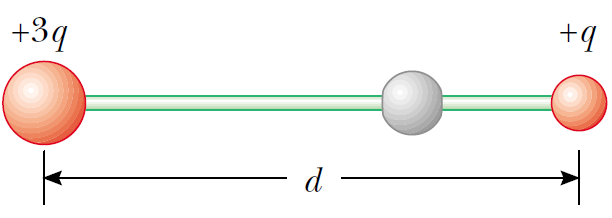
\includegraphics[scale=0.45]{FigureP23-10.png}
%\caption{Equilibrium of charge.}
%\label{Equilibrium}
%\end{figure}
%\nocite{*}
%\bibliographystyle{plain}
%\bibliography{PhysicsRef}
\end{document}
